\begin{blocksection}

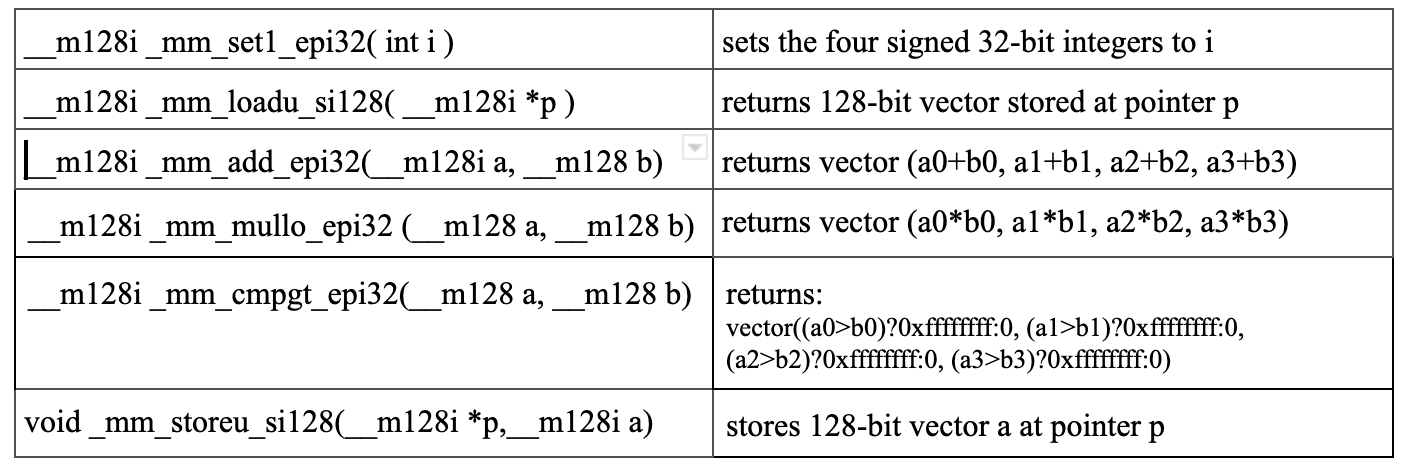
\includegraphics[width=\textwidth]{parallelism/simd}

\question
The following code uses loop unrolling to improve performance:
\begin{verbatim}
static void sum_unrolled (int *a) {
    int sum = 0;
    for (int i = 0; i < 16; i += 4) {
        sum += (a + i);
        sum += (a + i + 1);
        sum += (a + i + 2);
        sum += (a + i + 3);
    }
}
\end{verbatim}

\begin{parts}
    
\part
Implement the following function with a single SIMD instruction:
\begin{verbatim}
static void sum_unrolled_SIMD (int *a) {
    int sum = 0;
    int result[4];
    __m128i result_v = _mm_set1_epi32(0);
    for (int i = 0; i < 16; i += 4) {
        result_v = ___________________________________;
    }
    _mm_storeu_si128((__m128i*)result, result_v);
    sum = result[0] + result[1] + result[2] + result[3];
}
\end{verbatim}

\begin{solution}[0.5in]
\begin{verbatim}
result_v = _mm_add_epi32(result_v, _mm_loadu_si128((__m128*) (a + i) );
\end{verbatim}
\end{solution}
\end{parts}
    
\end{blocksection}